\section{Problema 3}
\subsection{Enunciado}
El problema es una generalización del juego $"$Uno Solo".
La idea es mover una pieza por vez $"$comiendo$"$ mediante un salto una ficha
adyascente siempre y cuando este vacío el siguiente casillero al adyacente.
El objetivo es eliminar todas las piezas, dejando solo una en el tablero.

\subsection{Soluci\'on}
El algoritmo presenta no solamente la existencia de un resultado, si no también el resultado del mismo (en caso de haber más se devuelve el primero encontrado).
La solución presentada utiliza el método de backtracking. La idea del algoritmo es ir recorriendo todas las fichas, corroborar que puedan realizar algún movimiento posible (dadas las reglas), realizarlo y ver si en esta instancia del tablero tiene solución. En caso de no tener solución, vuelve a la instancia anterior deshaciendo el movimiento antes mencionado y prueba con el moviemiento de esa ficha, si es que tiene, o la próxima ficha.
Ahora explicaremos más en detalle y la correctitud del algoritmo:\\
El caso base es cuando el tablero tiene una sola ficha, lo que significa que ya está resuelto. Por lo que devuelve true.
El caso recursivo recorre la lista de fichas , si la ficha está activa, es decir no fue comida, 
se prueban los cuatro moviemientos posibles, en caso de ser legal, realiza el movimiento, se apila el moviemiento, y se realiza la recursión sobre el tablero con el movimiento hecho.
Para mover la ficha, ideamos una clase tablero que contiene operaciónes y una estructura para facilitar y abstraer la matriz (el tablero) del algoritmo principal. Una de estas operaciones es la de mover, que básicamente cambia de valor en la matriz ,basándose en el movimiento previamente elegido, la posición de la ficha otorgada por parámetro. Queremos aclarar que la ficha obtenida no es una posición si no que es del tipo movimiento.
Este tipo movimiento nos permite almacenar la posición de la ficha y el movimiento (arriba, abajo, izquierda, derecha) a realizar. 
Volviendo al mover, esta operación, a partir del "movimiento" dado, calcula el lugar donde va a quedar la ficha, la ficha qué va a comer y preserva la posición anterior de la ficha movida. Para ello, en la matriz mantenemos los índices de la lista de fichas. Primero, recupero el índice de la ficha guardada en dicha matriz según su posición actual. Con este índice, actualizo en la lista de fichas, la nueva posición considerando el salto para "comer" y apilo el índice de la que comí en caso de que el recorrido elegido no sea el verdadero y tengamos que deshacer el movimiento mencionado. Por último, obtengo de vuelta el índice de la ficha comida, para poder marcarla como "comida" y en la matriz 
invalidar el índice, simulando la desaparición de la ficha.
Volviendo al algoritmo principal, después del movimiento, aplicamos recursivamente la solución en base a esta nueva versión del tablero.
Una vez que retorna un valor, true o false, hay que separar en casos.
En caso de que el valor sea veradero, implica que se encontró un resultado. Lo que implica el final del algoritmo. Recordemos que todos los movimientos fueron apilados de forma tal que solo resta devolver en orden esta pila.
En caso de que el valor sea falso, implica que no se encontró una solución para esta instancia de tablero. Por lo tanto, deshacemos dicho movimiento, borramos el movimiento fallido antes apilado y recorremos el siguietne moviemiento, ya se de esta ficha o la siguiente.
Para deshacer el movimiento, pasamos por parámetro el movimiento y el índie de la ficha movida, calculamos la posiciones para restaurar el movimiento. Esto es con el índice, actualizo en la lista de fichas la nueva posición, previamente calculando según la dirección. 
Actualizo los índice de la matriz, ya que ahora volvemos a tener las fichas que previamente fueron movidas y comidas. Y por último, marco como activa, es decir en juego, la última que comió.\\
Dado el algoritmo queremos demostrar la correctitud (informalmente) diciendo que ya que recorre las fichas, y sabemos que son finitas por precondición el algoritmo termina.
Por otro lado, sabemos que recorremos todos los posibles movimientos. Con esto quremos decir que no hay posibilidad no recorrida, así que si tiene solución, esta existe dentro
de todas estas posibilidades. Sin emargo, no es fuerza bruta ya que mide en tiempo constante, por cada instancia de tablero, aquellos movimientos que son posibles y reales (legales) podando ramas del árbol de posibilidades que sabemos que no pueden ser parte de la solución.\\
\\
Para un mejor entendimiento incluímos ejemplos de cómo resuelve el algoritmo:\\

{\huge Caso 3x3}
\begin {center}
\includegraphics[width=16cm]{./Solucion3x3.png}\\
\end {center}

{\huge Caso 4x4}
\begin {center}
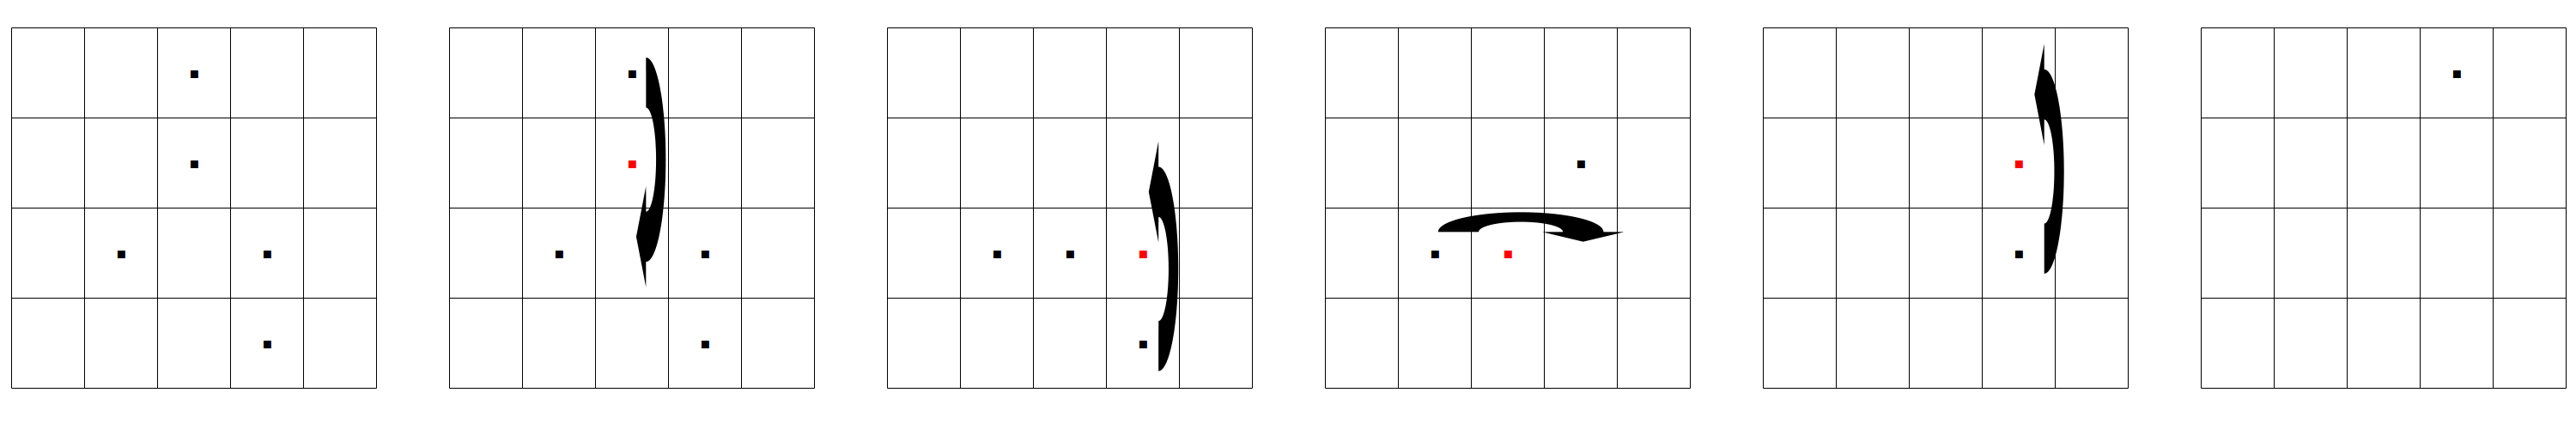
\includegraphics[width=16cm]{./Solucion4x4.png}\\
\end {center}

{\huge Caso 4x4 - Sin Solucion}
\begin {center}
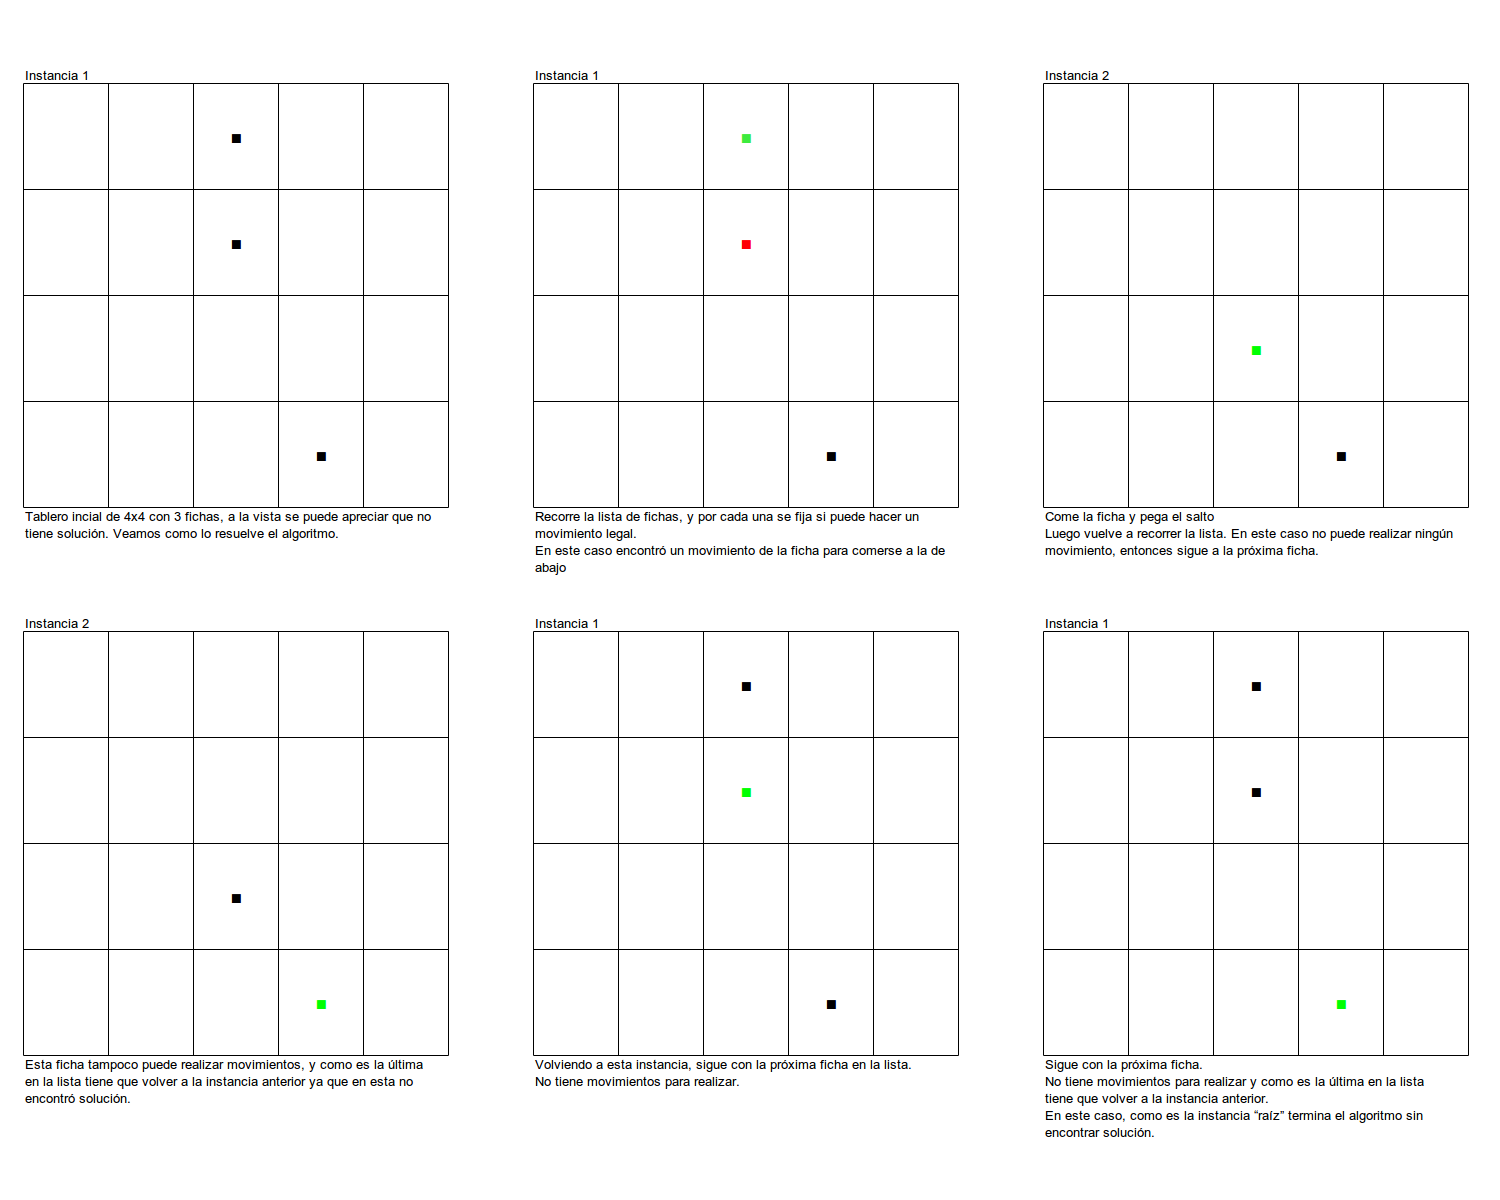
\includegraphics[width=20cm]{./SinSolucion4x4_2filas.png}\\
\end {center}


\subsection{Pseudoc\'odigo}

\begin{codebox}
\Procname{$\proc{solucion}$ (\textbf{in} $tablero$, \textbf{in/out} $pila$)}{encontrado}{Bool}
\li	\textbf{Si} cantidad de fichas == 1 \textbf{Hacer:} \Do
\li		return TRUE \End
\li	\textbf{Si no}  \Do
\li		\textbf{Para} cada ficha f en el tablero \Do
\li			\textbf{Para} cada movimiento m \Do
\li				\textbf{Si} es m movimiento legal \Do
\li					mov = crearMov(f,m)
\li					tablero = moverficha(mov)
\li					pila = apilarMovimiento(mov)
\li					encontrado = Solucion(tablero,pila)
\li					\textbf{Si} encontrado \Do
\li						return TRUE  \End
\li					tablero = deshacerMovimiento(mov,f)
\li					pila = desapilarMovimiento(mov) \End \End \End
\li		return FALSE \End
\end{codebox}

\mbox{}

Queremos volver a aclarar que el algoritmo presenta no solo si existe una solución si no también el camino, 
que tenemos guardado en la pila pasada por parámetro, solo faltaría imprimirlo. \\
Esta función de imprimir existe en el código pero para el contexto de esta sección decidimos no explicarlo
ya que no hace a la solución del enunciado.


\subsection{Análisis de complejidad}	

El algoritmo recorre una lista de fichas de longitud t.
Al recorrerla, si la ficha esta activa y el movimiento es legal (de los cuatro posibles). se realiza el movimiento y se tiene una ficha marcada como inactiva. 
En este momento, se intentara buscar una solucion a esta nueva instancia, que, 
 suponiendo el peor caso, por cada ficha mueve el tablero e intenta buscar una solución a este recursivamente.
Esta recursión vuelve a recorrer todas las fichas (discriminando entre las activas) y todos sus movimientos posibles hasta llegar al caso base de una sola ficha, siendo
la profundidad de t (quiere decir que maximo por cada instancia se llamara la solucion hasta agotar todas las fichas).
Entonces, queda:

\begin{codebox}
\li -Caso Base 
\li -Ciclo fichas \Do		   \RComment	O(t)
\li	Ciclo movimientos \Do	   \RComment	O(4)
\li		Paso Recursivo \Do \RComment	O($(4t)^{t-1}$)
	\End
 \End
Resto de las operaciones son O(1).
\end{codebox} 

\hbox{}
 
Entonces si la complejidad de los ciclos de recorrido de fichas y movimientos es de O(t) * O(4) = O(4t), y a su vez esta complejidad se efectua en cada paso recursivo, que como maximo tiene una profundidad de t, la complejidad total maxima quedara puesta en O(4t) 't' veces. \\
En otras palabras, como maximo, la lista de fichas y movimientos (O(4t)) se realizara hasta 
$"$comer$"$ todas las t fichas, dejando el siguiente producto:\\
$\prod\limits_{i=0}^t O(4t)$ = O($(4t)^t$)

\subsection{Tests y Gráficos}

En los siguientes gráficos, podemos apreciar que la complejidad del algoritmo varía notoriamente entre los tableros con solucion y aquellos que no tienen solución . \\


\begin {center}
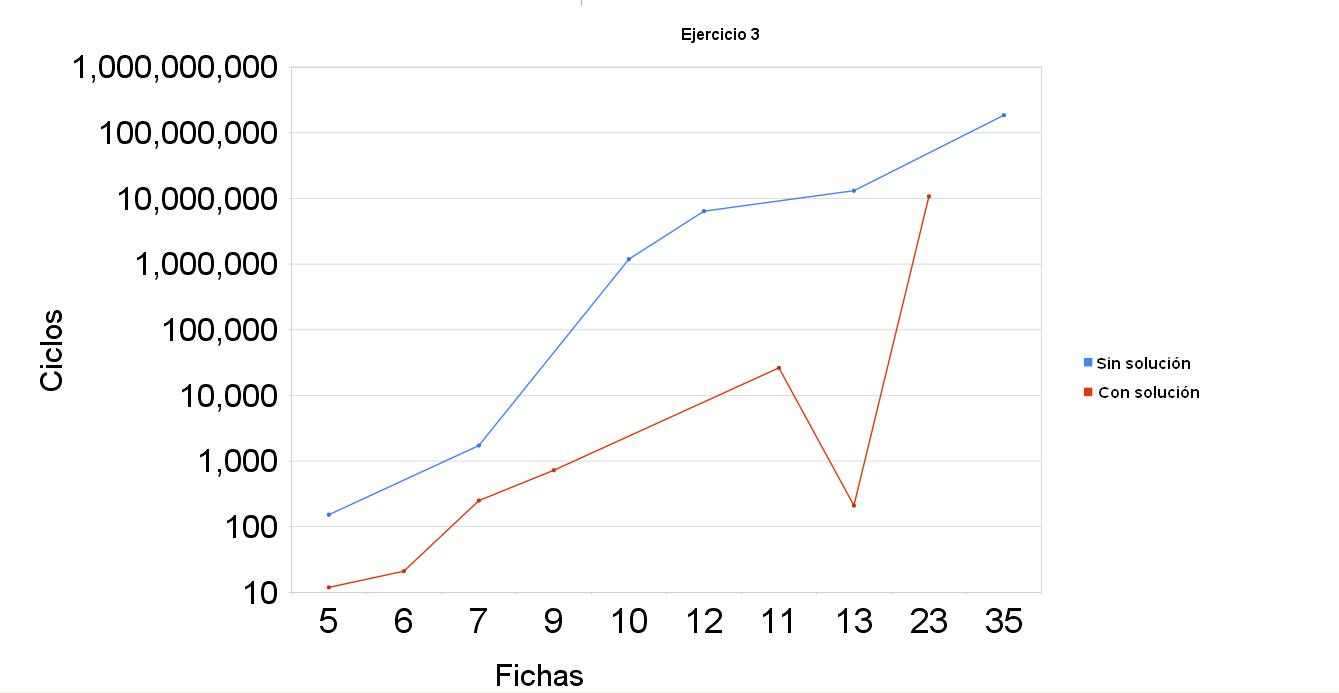
\includegraphics[width=16cm]{./graficoEj3.JPG}\\
\end {center}

Como podemos ver, aquellos que no tienen solución son de orden exponencial en la cantidad de fichas, ya que recorrerá todas ellas, y todos los movimientos posibles de ellas, sin poder ir descartando o \textit{podando} parte de la solucion. Esto es porque, si no tiene solucion, es que cada ficha o bien esta aislada o no puede llegar a comer a las otras, y el algoritmo no puede darse cuenta de eso, por lo que las analiza para encontrar soluciones, que nunca encontrará. \\
Lo contrario pasa con los tableros que si tienen solucion. Con un poco de azar (al comenzar a simular con la ficha correcta), podemos encontrar una solución en tiempo lineal, ya que si escogemos a la primera vez la que resuelve el problema, sólo tendremos que simular hasta que termine. En caso de que no encontremos a la primera vez la ficha indicada, la complejidad se torna un poco mayor, pero no alcanza el tiempo exponencial de los casos sin solución ya que, a diferencia de ellos, en éstos se van \textit{podando} soluciones, de forma tal que NO se recorren todas las fichas y sus movimientos posibles. \\
A continuación, mostramos las pruebas realizadas, donde sólo tomamos en cuenta tableros con hasta 35 fichas, ya que con más fichas, la simulación tarda demasiado en terminar (de hecho, los tableros más grandes tardaron bastante en finalizar), pero suponemos en forma teórica que el crecimiento seguirá de la misma forma, ya que no podemos analizarlo en forma práctica. \\

\begin {center}
\includegraphics[width=12cm,height=9.5cm]{./testConSolEj3.png}\\
\end {center}

\begin {center}
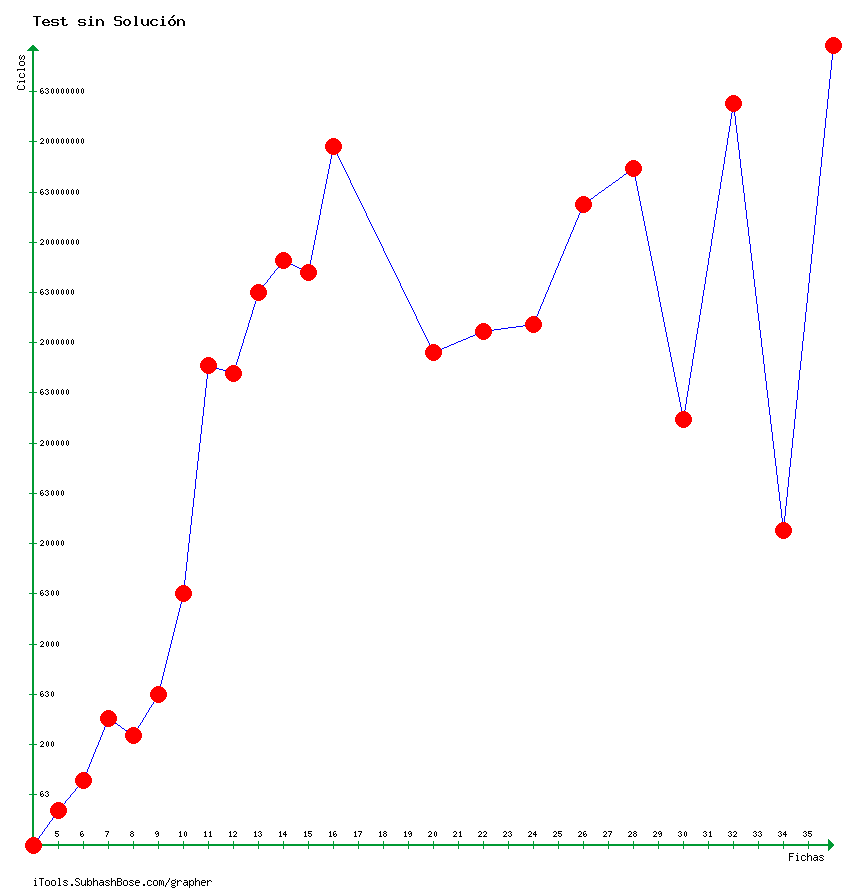
\includegraphics[width=12cm,height=9.5cm]{./testSinSolEj3.png}\\
\end {center}

Con estos gráficos podemos notar que no solo la cantidad de fichas afecta al tiempo, si no también la posición de las mismas. Con esto queremos decir, 
que existen casos en donde si bien no tiene solución, podemos darnos cuenta más rápido. Los casos son aquellos en donde no existe ningún movimiento para realizar
de entrada (ejemplo: todo el tablero lleno de fichas), y esto aplicado recursivamente.\\
Podemos llegar a predecir que la complejidad mínima, sin contar el caso de que haya una ficha o ninguna, es O(t), siendo t: la cantidad de fichas.


\subsection{Conclusiones}
Concluimos que era necesario utilizar una metodología como la de backtracking para la realización de este algoritmo, ya que, para encontrarle una solución a las diferentes entradas se necesitaba ir recorriendo todos los movimientos posibles de las fichas y podando casos que no sirvan para la resolución.
Al ir cualculando siempre instancias diferentes del tablero a solucionar, resolverlo con programación dinamica no hubiese sido lo mejor ya que no habia resultados que guardar para no volver a procesarlos.
Si bien el algoritmo de backtracking puede llegar a ser muy ineficiente (ver Complejidad), eso solo ocurre
cuando no puedo descartar ninguna de las ramas, caso bastante patológico e improbable de ocurrir, que se suele dar cuando la cantidad de fichas es mayor a la cantidad de espacios vacios.
También cabe destacar que si bien la complejidad es alta (es exponencial), para los casos donde las fichas son menos que los espacios vacios y tiene solución, la complejidad esta muy por debajo de la cota máxima.
